\input ../SlidePreamble
\input ../preamble

\begin{document}

{\Huge

  \centerline{\bf TTIC 31230, Fundamentals of Deep Learning}
  \bigskip
  \centerline{David McAllester, Autumn 2024}


  \vfill
  \centerline{\bf Diplomacy}
  \vfill
  \vfill

\slide{Cicero Plays Diplomacy}

{\bf Human-level play in the game of Diplomacy by combining language models with strategic reasoning}, (Meta, November 2022)

\vfill
Players engage in secret negotiaions to conspire to take over the world.

\vfill
\centerline{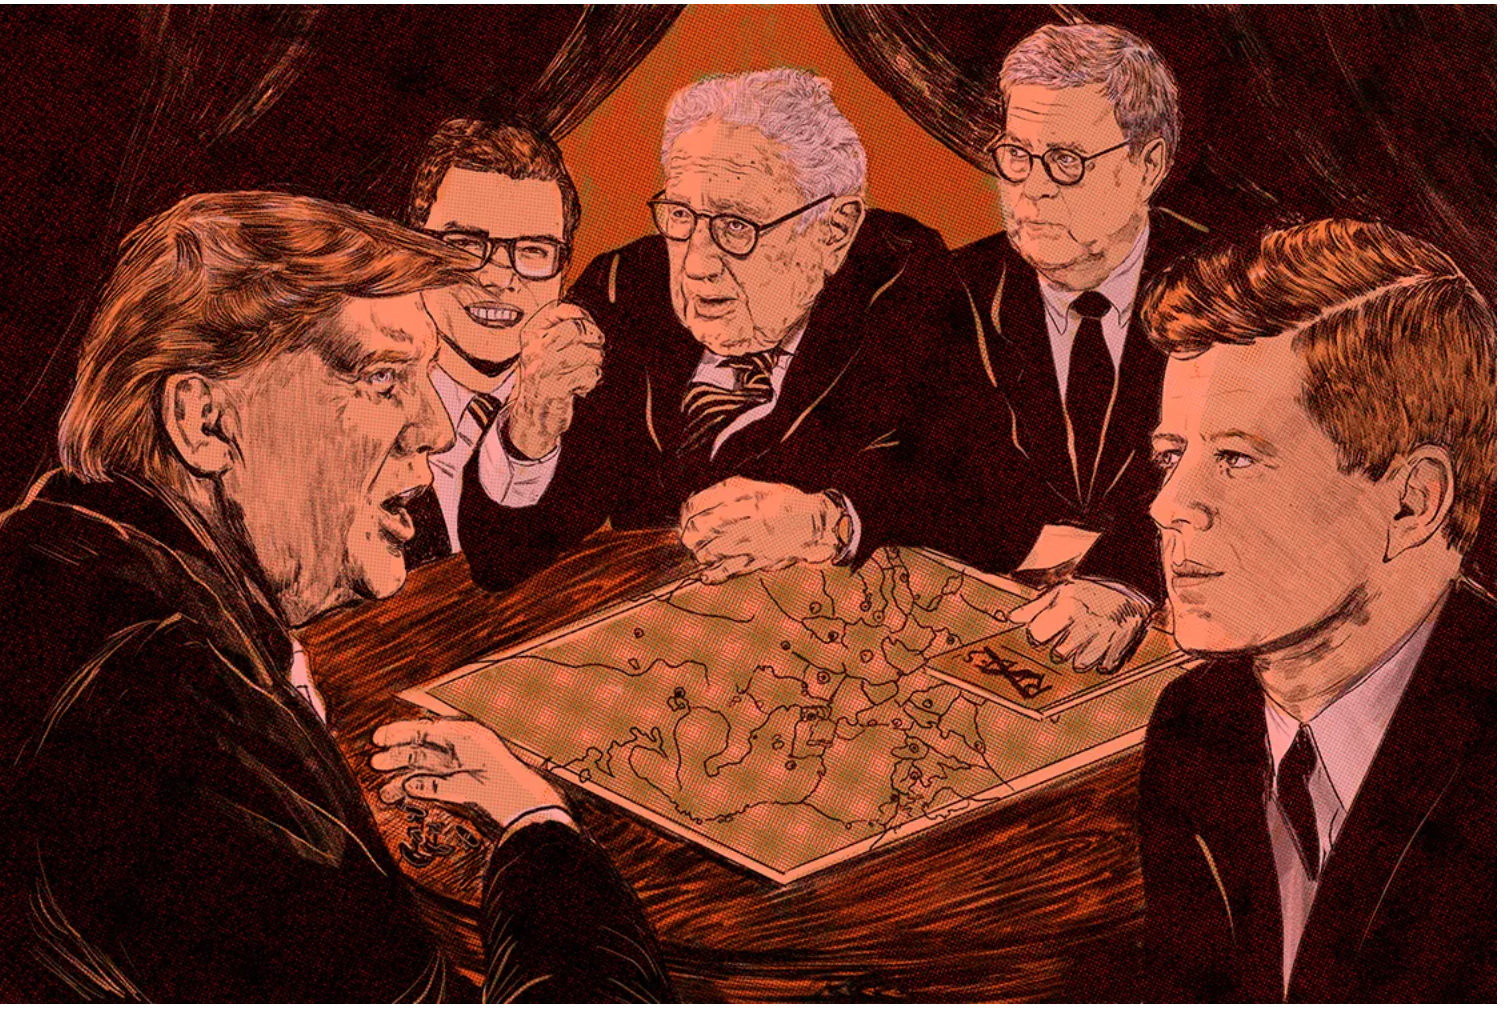
\includegraphics[width = 4.0in]{\images/Diplomacy02}\hfill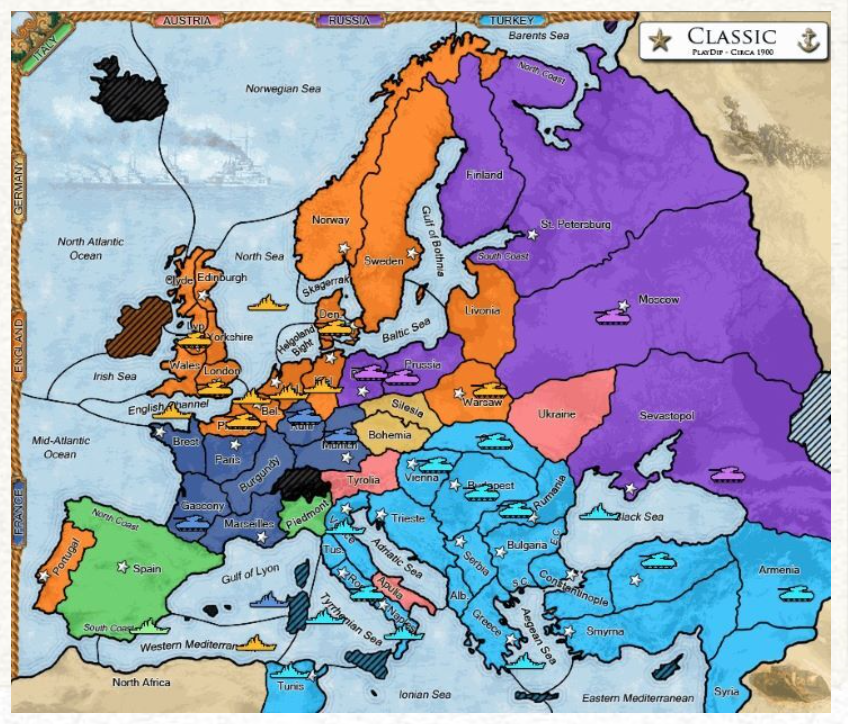
\includegraphics[width = 3.0in]{\images/Diplomacy01}}

\slide{Cicero Plays Diplomacy}

\vfill
\centerline{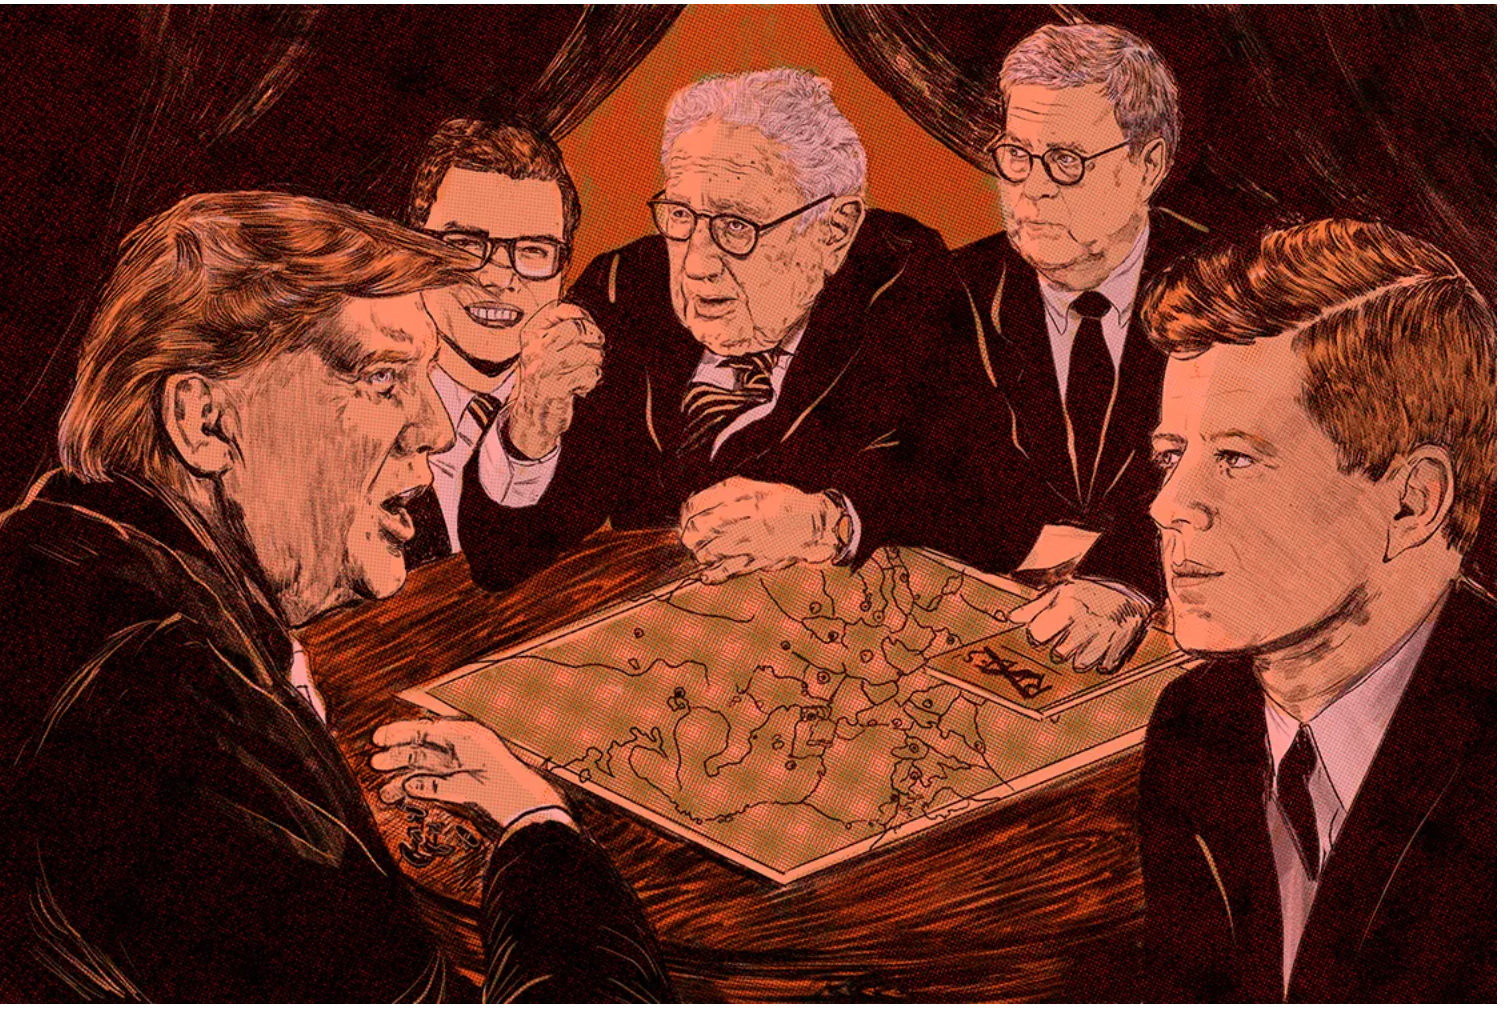
\includegraphics[width = 3.0in]{\images/Diplomacy02}\hspace{4em}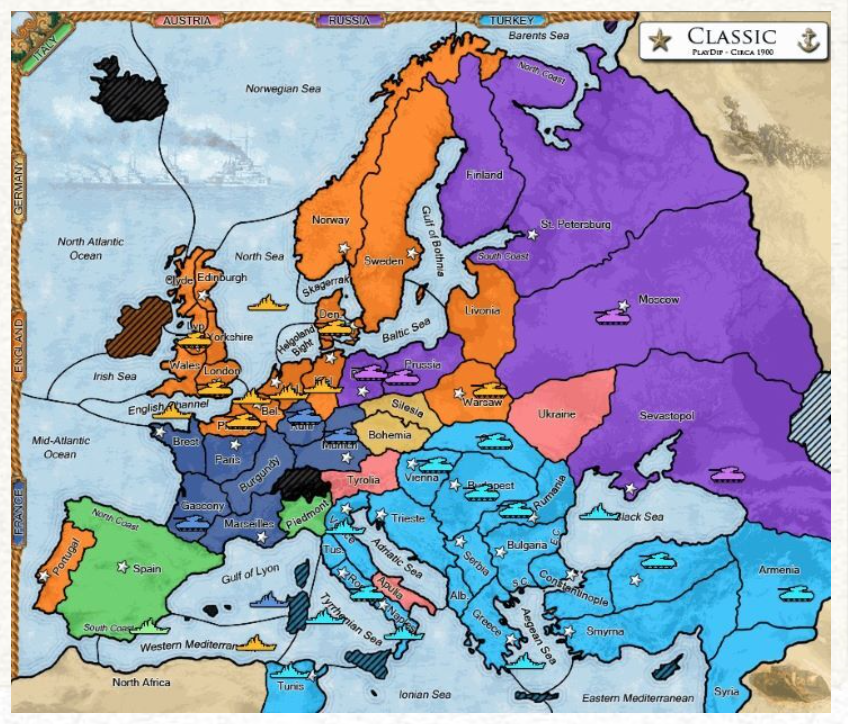
\includegraphics[width = 2.0in]{\images/Diplomacy01}}

\vfill
The play consists of a sequence of ``turns''.  In each turn each player converses with the others using a private messaging system.  After some time the messaging ends and each player submits orders to their generals.  The orders are revealed simultaneously. Promises can be broken.  The orders determine a state transition on the game board (no dice).


\slide{Cicero Plays Diplomacy}

Cicero is an AI agent that plays Diplomacy with humans.  It is rated in the top 10\% of human players.

\slide{Overall Comments}

The natural language aspect of the game turns out be the easy part.

\vfill
In the game of Diplomacy the set of possible orders that can be given for a given board configuration is highly constrained.

\vfill
This greatly facilitates interpreting and generating language.

\vfill
The hard part is ``solving'' the formal game (selecting proposed actions during negotiation and selecting final orders).

\slide{GPT-4 Cannot Play Formal Games}

It is worth noting that GPT-4 cannot play chess or Diplomacy --- it seems GPT-4 cannot effectively plan actions in games defined by formal rules.

\slide{Game Theory: Nash Equilibria}

The game theory of multi-player games, even without negotiation, is complicated.

\vfill
(Without negotiation) a Nash equilibrium is a policy $\pi_i$ for each player $i$ such that each player is playing best-response under
the policies of the other players.

$$\pi_i = \argmax_{\pi_i} V_i(\pi_i,\pi_{-i})$$

\vfill
Here $\pi_{-i}$ is the set of policies for all players other than $i$.

\slide{Planning in a Multi-Player Game}

One can plan in a multi-player game by assuming that the players will all find the same Nash equilibrium and that one can find
this equilibrium by searching for it.

\vfill
One then plays one's own best response in the Nash equilibrium.

\vfill
A form of equilibrium search is done in Cicero.

\slide{Negotiation: Correlated Nash Equilibria}

At the end of negotiation it is natural to search for policies $\pi_1,\ldots,\pi_n$ that form a Nash equilibrium
conditioned on the text of the negotiation.

\vfill
In the presence of negotiation (or other partially observable ``signal'') this is called a correlated equilibrium
because the negotiation introduces correlations between the actions of different players.


\slide{Imitation Learning}

Cicero uses both an imitation-trained model and a self-play-trained model.

\vfill
For imitation learning Cicero uses 
a dataset of over 12 million games from WebDiplomacy including messages exchanged between players. (WebDiplomacy deidentified Player accounts).


\newcommand{\act}{\mathrm{act}}
\newcommand{\mess}{\mathrm{mess}}
\newcommand{\im}{\mathrm{im}}

\slide{Imitation Learning}

We define an ``action'' to be a set of orders given to generals.  The state transition is determined by an end-of-turn action for each player.

\vfill
Cicero continuously predicts all player's final actions during the negotiation phase (including its own).

\vfill
$$\im^* = \argmin_\im\;E_{(x_i,a_j) \sim \train}\left[-\ln P_\im(a_j|x_i)\right]$$

\vfill
``im'' stands for ``imitation''.

\slide{Imitation Learning}

$$\im^* = \argmin_\im\;E_{(x_i,a_j) \sim \train}\left[-\ln P_\im(a_j|x_i)\right]$$

\vfill
$x_i$ is taken from a time during negotiation and
consists of all past board positions and the previous messages in this negotiation visible to player $i$.

\vfill
$a_j$ is the action actually taken at the end of that round by player $j$.

\vfill
If $j = i$ this is an imitation action policy for $j$.

\vfill
If $j \ne i$ this is $i$'s imitation belief about $j$ intended action.


\slide{Learning from Self Play}

Cicero trains a value function that assigns a value $V_i(b)$ giving an estimate of the value that player $i$ receives 
given board position $b$.

\vfill
As games are played the value function can be trained with standard methods --- Bellman error and replay buffers.

\slide{Learning from Self Play}

During self-play Cicero is playing all of the players.

\vfill
Before sending each negotiation message Cicero samples 30 actions for each player $i$
from the imitation action predictions $P(a_i|x_c)$.

\vfill
Cicero then searches for ``equalibrium policies'' $\pi_1,\ldots \pi_n$ where each $\pi_i$ is selecting one of the 30 selected actions for that agent.

\slide{Learning from Self Play}

Cicero then optimizes policies $\pi_1,\ldots,\pi_n$ according to a piKL best-response objective
where $\pi_{-i}$ is the collection of policies other than $\pi_i$.

\vfill
$$\pi_i^* = \argmax_{\pi_i}\;V_i(\pi_i,\pi_{-i}) - \lambda KL(\pi_i,P_\im(a_i|x_c))$$

\vfill
At the end of the negotiation each player draws an action from their policy.

\slide{Playing with Humans}

During negotiation
Cicero uses self play to estimate the policies (intentions) of the Human players.


\vfill
The final actions are (of course) made by Cicero and the human players.

\slide{Imitation Message Generation}

Cicero has a model $P_\mess(y|s,r,a_s,a_r,x_s)$ where
where $y$ is the English text of the message, $s$ is the message sender, $r$ is the message recipient,
$a_s$ is the action taken by the message sender and $a_r$ is the action
taken by the message receiver at the end of the turn (in the future).

\vfill
$x_s$ consists of all past board positions and the previous messages visible to the sender in the current negotiation.


\slide{Imitation Message Generation}

{\huge
$$\mess^* = \argmin_\mess\;E_{\{(x,s,r,y,a_s,a_r) \sim \train\}} \left[-\ln P_\mess(y|s,r,a_s,a_r,x_s)\right]$$
}

\slide{Overall Comments}

The natural language aspect of the game turns out be the easy part.

\vfill
In the game of Diplomacy the set of possible orders that can be given for a given board configuration is highly constrained.

\vfill
This greatly facilitates interpreting and generating language.

\vfill
The hard part is ``solving'' the formal game (selecting negotiation proposals and final orders).

\slide{END}

}
\end{document}
